\documentclass[letterpaper,11pt]{article}
\usepackage{tabularx}
\usepackage{amsmath}
\usepackage{graphicx}
\usepackage[margin=1in,letterpaper]{geometry}
\usepackage[final]{hyperref}
\usepackage{lineno}
\usepackage{siunitx}
\usepackage{xspace}
\usepackage{enumitem}% http://ctan.org/pkg/enumitem
%%%%%%%%%%%%%%%%%%%%%%%%%%%%%%%%%%%%%%%%%%%%%%%%%%%%%%%%%%%%%%%%%%%%%%%%

\setlist[description]{labelindent=25pt,style=multiline,leftmargin=2.5cm}
\linenumbers
\newcommand{\ws}{\ensuremath{s_\mathrm{w}} \xspace}
\newcommand{\wdam}{\ensuremath{d_\mathrm{w}} \xspace}
\newcommand{\psoc}{\ensuremath{p_\soc} \xspace}
\newcommand{\soc}{\ensuremath{\mathrm{SoC}} \xspace}
\newcommand{\sob}{\ensuremath{\mathrm{SoB}} \xspace}
\newcommand{\dave}{\ensuremath{d_{\mathrm{ave}}} \xspace}
\newcommand{\dswing}{\ensuremath{d_{\mathrm{swing}}} \xspace}
\newcommand{\dphys}{\ensuremath{d_{\mathrm{phys}}} \xspace}
\newcommand{\dholy}{\ensuremath{d_{\mathrm{holy}}} \xspace}
\newcommand{\armor}{\ensuremath{a}\xspace}
\newcommand{\lvl}{\ensuremath{l}\xspace}
\newcommand{\pwf}{\ensuremath{p_{\mathrm{WF}}} \xspace}
\newcommand{\dr}{\ensuremath{DR(\%)} \xspace}
\hypersetup{
	colorlinks=true,       % false: boxed links; true: colored links
	linkcolor=blue,        % color of internal links
	citecolor=blue,        % color of links to bibliography
	filecolor=magenta,     % color of file links
	urlcolor=blue         
}
%\setlength{\parindent}{0pt} 

%%%%%%%%%%%%%%%%%%%%%%%%%%%%%%%%%%%%%%%%%%%%%%%%%%%%%%%%%%%%%%%%%%%%%%%%

\begin{document}
	
	\title{The Mathematics of Ret Paladin in BCC}
	\author{Swedge}
	\date{\today}
	\maketitle
	
	\begin{abstract}
		This document details considerations relevant to a Burning Crusade Classic (BCC) retribution paladin's rotation and calculations for relative damage outputs of various rotations, in an attempt to help players understand paladin rotations and to ensure the rotations we use are the formally optimal ones.
	\end{abstract}
	
	%%%%%%%%%%%%%%%%%%%%%%%%%%%%%%%%%%%%%%%%%%%%%%%%%%%%%%%%%%%%%%%%%%%%%%%%
	\section{Introduction}
	
	Retribution paladin in BCC relies heavily on ``seal twisting'' to increase the class's damage output.
	This technique of swinging with two active seals was an artefact of ``spell batching'' in retail BC, where as an optimisation the server processed batches of actions that would be evaluated together.
	
	In BCC, the batch size was greatly reduced, but some seals were changed to persist for a very short time after switching to another seal.
	This allows the paladin to change seals very shortly before a swing, and to have both seals active. For reasons we will cover when looking at the paladin's abilities, this results in some multiplicative damage effects over strictly additive ones, significantly increasing the paladin's damage output.
	
	In this document, we will first examine the ret paladin's abilities and the buffs we commonly utilise.
	We will then define expected damage outputs as a relative fraction of weapon damage, starting with simple situations and later taking into account more complex considerations.
	This allows us to somewhat ignore what gear the ret is using, with some notable exceptions.
	
	This is, of course, no substitute for a sim - but it can help theorycrafters to some extent quantify the expected damage output and value of different rotations, and perhaps to find new rotations that had been previously considered unviable.
	
	%%%%%%%%%%%%%%%%%%%%%%%%%%%%%%%%%%%%%%%%%%%%%%%%%%%%%%%%%%%%%%%%%%%%%%%%
	\section{Assumptions}
	We make the following assumptions that generally hold in a PvE raiding scenario:
	\begin{itemize}
		\item the ret is lvl 70
		\item the ret is in a raid group with an enhancement shaman casting Windfury Totem with $100~\%$ uptime
		\item the ret is attacking a boss enemy at lvl 73
		\item the ret's weapon skill is maxed out at 350
		\item the ret is hit-capped, and has sufficient hit rating to remove misses from the attack table
		\item the ret is hitting the target from behind, so cannot be parried
		\item the ret is \emph{not} dodge-capped at $6.5\%$, meaning there is some finite chance for their attacks, seals, and some abilities to be dodged 
	\end{itemize}
	
	%%%%%%%%%%%%%%%%%%%%%%%%%%%%%%%%%%%%%%%%%%%%%%%%%%%%%%%%%%%%%%%%%%%%%%%%
	\section{The BCC Combat System}
	In this section we detail certain facets of the BCC combat system and character statistics relevant to a ret paladin's performance.
	
	\subsection{The Attack Table}
	Basic attacks in TBC are determined as a single random roll on the server.
	This means that every possible outcome for the attack is weighed together in one roll (as opposed to e.g. a multiple roll system that first evaluates the probability of an attack to
	hit or miss, and then subsequently makes a second independent roll upon a hit to evaluate critical strike chance, glancing chance etc).
	
	Each outcome of the single roll is assigned a certain precedence, such that higher precedence outcomes have the capability under certain conditions to ``push'' lower precedence outcomes off of the attack table.
	These outcomes are:
	\begin{description}
		\item[miss] the attack misses the target and is negated.
		\item[dodge] the target dodges and the attack is negated.
		\item[parry] the target parries the attack, negating the attack and hasting their autoattack timer. Parries can only occur when attacking the target from the front.
		\item[glance] when the target is three levels or more higher than the attacker, there is a chance for the attack to be a glancing blow, which deals reduced damage. The damage reduction on the attack is rolled uniformly between $15 - 35 \%$, for an average reduction of $25\%$. When the attacker is three levels lower than the target, the chance for a glancing blow to occur is $24\%$.
		\item[block] the target blocks the attack, reducing the damage taken from the attack in accordance with the incoming damage and the target's \emph{Block Value} statistic.
		\item[crit] the attack is a critical hit, dealing a base of $200\%$ the regular damage. Critical strike damage can be modified by gear and talents.
		\item[hit] the attack is a hit, dealing regular damage.
	\end{description}
	In practical PvE scenarios, the ret is hitting the target from behind.
	As such, the block and parry outcomes are removed from the attack table.
	The miss and dodge outcomes can be reduced or eliminated entirely through appropriate gear and talents.
	In our scenario, the target enemy is three levels higher than the ret and therefore glancing blows must be accounted for in the attack table.
	Glancing blow chance cannot be reduced.
	
	\subsection{The Global Cooldown (GCD)}
	The Global Cooldown or GCD is a period following an ability cast (and not a swing or seal hit) where no further casts are possible.
	The base duration of the GCD is 1.5s, but it can be reduced by Spell Haste.
	Ret paladin's commonly acquire Spell Haste through the Shaman's Bloodlust ability and the Leatherworker's Drums of Battle, which together reduce the GCD to 1.1s.
	
	The GCD is of particular importance to a ret paladin's ability to seal twist.
	In order to twist e.g. a SoC into a SoB, the SoC ability (which is typically not the seal at the start of the swing, favouring SoB under most scenarios) must be cast more than a GCD before the swing timer completes such that the paladin can cast the secondary seal before the swing completes and the attack is made.
	
	We also note that the Crusader Strike ability is not a cast and does not benefit from Spell Haste, meaning the GCD following its use is \emph{always} 1.5s.
	
	\subsection{Internal Cooldowns (ICD)}
	Internal Cooldowns refer to the time period where a given spell or ability cannot proc after proccing.
	
	The relevant ICDs to a ret paladin are:
	\begin{itemize}
		\item Seal of Command, which has a 1s ICD to prevent it from proccing on both an autoattack and Windfury Attack on the same swing
		\item Windfury Attack itself, which has a very short ICD to prevent it from proccing on both an autoattack and a Seal of Command attack.
	\end{itemize}

	\subsection{Armor}
	Armor is a stat that reduces the amount of physical damage received by a target.
	All targets have an armor value, and BCC bosses typically have either 6200 or 7700 armor.
	The target's level also influences the amount of damage reduction that a given level of armor will provide.
	The damage reduction formula for targets over level 60 is given as
	\begin{equation}
		\dr = 100 \frac{\armor + 1}{467.5 \lvl -22167.5}
	\end{equation}
	where \armor is the target's armor value, and \lvl is the target's level.
	A significant proportion of a paladin's damage is physical, and so the target's armor level must be considered when evaluating rotations.
	
	\subsection{Spell Resistance}
	In BCC, spells have a chance to be resisted either fully, such that the spell is nullified, and/or partially in the case of many damaging spells.
	Partial resists result in the spell's damage being resisted by either $25\%$, $50\%$, or $75\%$.
	The chance to be resisted is dependent on the level difference between the caster and the target, the caster's Spell Penetration stat, and the target's resistance to the relevant school of magic.
	
	Some of the ret paladin's offensive seals are partially implemented as spells that do holy damage.
	They cannot be fully resisted, but they can be partially resisted.
	Holy is not a school of magic for which spell resistance can be acquired.
	Therefore the chance for a seal to be partially resisted is therefore entirely dictated by the level difference between the caster and target.
	
	Against raid bosses, the level difference is always equal to 3.
	In this case, the probabilities for a seal to be partially resisted are given in Table \ref{table:1}.
	\begin{table}
		\centering
			\begin{tabular}{r | l}
				Resistance (\%) & Probability \\
				\hline \hline
				0 & 0.82 \\
				25 & 0.13 \\
				50 & 0.04 \\
				75 & 0.01 \\
				100 & 0 \\
				\hline
			\end{tabular}
	    	\caption{Probabilities for spell partial resists against a Boss target}		
			\label{table:1}
	\end{table}
	Integrating these values gives an average damage resistance against a ret paladin's seals of $6\%$.

	\subsection{Hit Rating and Hit Chance}
	Against level 73 (or Boss level) targets, wielders of only a single weapon need a total of $9\%$ Hit Chance to never miss a target.
	Hit rating is found on gear, and increases Hit Chance.
	At level 70, 15.8 Hit Rating increases your Hit Chance by $1\%$. 
	Paladins have access to the talent \emph{Precision}, which increases the Hit Chance and Spell Hit Chance by $3~\%$.
	The Balance specialisation of the Druid class has access to the talent Improved Faerie Fire, which increases the targets chance to be hit by $3~\%$ when affected by the Faerie Fire debuff.
	In most raiding scenarios, the ret paladin must therefore acquire at least 48 Hit Rating from their gear to attain an additional $3\%$ Hit Chance in order to fully remove the chance to miss from the attack table.
	This is almost always very trivial, and so we do not need to consider miss chance in our considerations.
		
	\subsection{Expertise Rating and Expertise}
	When melee attacking a target 3 levels higher, a player has a base $6.5\%$ chance to be dodged.
	As parries can only occur when attacking the target from the front, and we attack the target from behind, parries are usually not present in the attack table.

	Each point of Expertise reduces the target's chance to dodge or parry an attack by $0.25\%$.
	Expertise Rating is found on gear.
	At level 70, 3.9 points of Expertise Rating are required to give one point of Expertise.
	As such, a player requires 26 Expertise to totally remove dodge chance from the attack table.
	
	Ret paladins do not typically take any talents that provide Expertise.
	As such, most races of paladin must acquire 102 points of Expertise Rating from their gear in order to reach 26 Expertise.
	Humans have a racial passive that provides them with 5 Expertise when using a sword or mace.
	Human rets when using the appropriate weapon only require 82 points of Expertise Rating in order to reach 26 Expertise.
	
	Because Expertise Rating is relatively scarce on gear, most paladins retain some chance to be dodged even when wearing excellent or even optimal gear.
	For instance, a non-human ret can only acquire a maximum of 95 Expertise Rating in phase two of BCC, and therefore retains a $0.5\%$ chance to be dodged.
	Due to Expertise typically being available on gear only in large increments, it is not optimal for human rets in phase two to run a gear setup that fully eliminates dodge chance.
	
	As we will cover when looking at the ret paladin's abilities later in this document, Seal spells also have a chance to be dodged.
	Because of the chained nature of a paladin's damage rolls, ret paladin's benefit more from Expertise than any other melee class in BCC.
	
	\subsection{Attack Power (AP)}
	Attack Power increases base melee damage per second by 1 point for every 14 Attack Power.
	When considering rotations, this stat is of note because Windfury Attacks from an enhancement Shaman's Windfury Totem have a bonus to Attack Power.
	Therefore rotations that favour twists and SoC swings will benefit \emph{very slightly} from the extra AP on those attacks because SoC can proc Windfury Attack.
	
	\subsection{Critical Strike Chance}
	Critical strike chance is the chance for an attack to critical strike.
	It is relevant to evaluating rotations because of an interaction between the Libram of Avengement item and the Judgement of Blood ability (detailed later).
		
	\subsection{Critical Strike Damage}
	Critical Strike Damage accounts for any improvements to the base $200\%$ critical strike damage.
	Ret paladins without exception should use the Relentless Earthstorm Diamond as their helmet's meta gem, which provides $3~\%$ increased critical damage.
	As such, a typical critical strike for a ret paladin will do $206\%$ of the base damage.
	
	\subsection{Spellpower}
	A player's spellpower increases the damage of their spells, by a multiple of their total spellpower multiplied by the spell's spell damage coefficient.
	As ret paladin's optimally do not use any gear that includes spellpower, we ignore it in this document.
	
	%%%%%%%%%%%%%%%%%%%%%%%%%%%%%%%%%%%%%%%%%%%%%%%%%%%%%%%%%%%%%%%%%%%%%%%%
	\section{Ret Abilities}
	We will now detail the most important abilities to a ret's rotation.

	\subsection{Autoattacks and Windfury Attacks}
	The plurality of a ret's damage output comes from autoattack damage and Windfury Attacks.
	A shaman's Windfury Totem has a short internal cooldown, that prevents a melee attack and a SoC attack (detailed later) from proccing on the same swing.
	As our hypothetical ret is hit-capped, misses are removed from the attack table, but they are
	not dodge-capped, so dodges will still be present in accordance with the ret's expertise stat.
	Autoattacks and Windfury Attacks can both, of course, be dodged.
	
	Windfury Attacks get a bonus to AP, so they are more damaging than regular attacks by a constant damage factor.
	This means that as the ret's total amount of AP goes up, the difference in the average damage between a regular attack and a windfury attack goes down.
	
	Windfury attacks caused by the max rank Windfury Totem get a bonus to attack power of 445AP, which is usually increased by $15~\%$ by taking one rank in Improved Weapon Totems talent in the Enhancement tree for a total of 511.75AP.
	This adds approximately 41.3dps to the attack, meaning that the damage added to the attack is dependent on the weapon's base speed.
	For example, for $\ws = 3.6~\mathrm{s}$ the attack's damage is increased by approximately 131 damage.
	The formula to calculate this extra damage is given by:
	
	\begin{equation}
		d = \frac{578.5 \ws}{14}
	\end{equation}
	
	\subsection{Seals and Judgements}
	Seals are 30s duration buffs the paladin casts on themselves.
	The effect of a seal can be expended by using the Judgement ability to produce a damaging action or to cast a debuff on the target.
	Judgement is notably off the GCD, meaning it can be cast while the GCD is ticking.
	
	Retribution paladins do a significant portion of their damage as holy damage through offensive seals that enhance their auto-attacks.
	The two most relevant to ret rotations, Seal of Command and Seal of Blood, are implemented in TBC in ways that are not strictly like spells or like autoattacks.
	We will detail these seals and their behaviours below.
		
	\subsubsection{Seal of Command (SoC)}
	This ability gives the paladin a chance to do $70\%$ of their weapon damage as holy on their swing.
	The chance is determined by the base weapon speed of the paladin's weapon, and is normalised at 7 procs per minute (PPM).
	The proc chance of SoC is therefore given by:
	
	\begin{equation}
		\psoc = \frac{7 \ws}{60}
	\end{equation}
	where \ws is the base swing speed of the paladin's weapon in seconds.
	This is the primary reason that rets favour slow weapons - under 0 haste and neglecting windfury hits, a quick weapon procs SoC on average 7 times for low damage due to the PPM normalisation, while a slow weapon procs SoC 7 times on average per minute for high damage.
	The proc chance is unchanged by haste effects, meaning that one can proc SoC well over 7 times per minute while under high haste.
	There is no limit on how many times SoC can proc in any given minute.
	
	SoC can be partially resisted unlike most spells, and it has a spellpower coefficient (meaning it benefits from spellpower on gear).
	It is to some extent implemented as an attack that does holy damage, meaning that it can proc windfury.
	It has an internal cooldown (ICD) of 1s, meaning that it cannot be procced on e.g. both melee hits in a windfury attack.
	
	SoC \emph{lingers}, meaning it persists for 400~ms after the paladin casts another seal.
	As such, it can be used as the first seal in a twist attempt.
	
	\subsubsection{Judgement of Command}
	When the ret has SoC active, the Judgement ability will deal an amount of holy damage to the enemy, which is increased against incapacitated targets.
	Because SoC is the best seal to start a twist from, its judgement is never used in PvE content.
	As such we will not go into detail on its damage, or any related libram effects that improve SoC's judgement.
	
	\subsubsection{Seal of Blood (SoB)}
 	This seal gives the paladin a $100 \%$ chance to do $35 \%$ of their weapon damage as holy on their swing, at the cost of the paladin losing health equal to $10 \%$ of the damage inflicted.
 	SoB is mostly a spell, and can be partially resisted, but it has no spellpower coefficient.
 	It is not an attack, and therefore it cannot proc windfury.
 	SoB has no ICD, meaning it can proc on both hits of a windfury attack.
 	Seal of blood does not linger, meaning that it can only be twisted into, and not as the first seal in a twist.

	\subsubsection{Judgement of Blood}
	When the ret has SoB active, the Judgement ability will deal 295 to 325 Holy damage at the cost of health equal to $33 \%$ of the damage caused.
	The best Libram for rets in TBC is available starting in phase 1, the Libram of Avengement.
	
	\begin{figure}[ht] 
		\centering 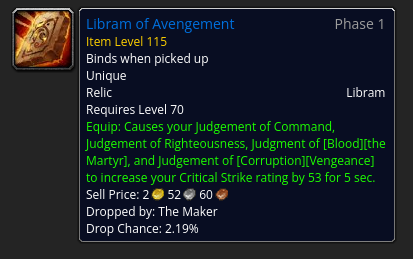
\includegraphics[width=0.44\columnwidth]{figs/libram_of_avengement.png}
%		\caption{\label{fig1}}
	\end{figure}
	
	This libram causes several judgements, including Judgement of Blood, to increase the ret's critical strike rating by 53 for 5 seconds.
	As such, any rotations that provide the ret time to judge blood will affect the expected damage of the ret's attacks and seals for a subsequent 5 seconds, and critical strike chance must be included in any rigorous damage projections.
	
	\subsection{Crusader Strike (CS)}
	CS is an instant cast strike that deals $110 \%$ weapon damage to the target, and refreshes all judgements on the target.
	It has a 6 second cooldown.
	
	\subsection{Consecrate}
	...
	
	\subsection{Exorcism}
	...
	
	%%%%%%%%%%%%%%%%%%%%%%%%%%%%%%%%%%%%%%%%%%%%%%%%%%%%%%%%%%%%%%%%%%%%%%%%
	\section{Swing Damages}
	Now that we have detailed BCC's combat system and its facets relevant to a ret paladin's damage output, we may now turn to the task of quantifying the projected damage of various actions a ret paladin can take. For the purposes of comparing rotations, it is useful to normalise the projected damage to the weapon damage of the ret paladin's weapon. This allows us to neglect gear dependencies to some extent.
	
	\subsection{Naked Swing}
	A naked swing is defined as a swing the paladin takes that has no Seal active.
	It is affected by the following:
	\begin{itemize}
		\item windfury procs
		\item dodge chance
		\item boss armor value
	\end{itemize}
	
	The projected damage of a naked swing is given by
	\begin{equation}
		d = 
	\end{equation}
	
	
%	\subsection{Simple Case}
%	We assume no windfury buffs, and neglect dodge chance and armour/partial resists.
%	
%	\subsubsection{SoB swing}
%	\noindent
%	Swinging with SoB up we get an average swing damage of
%	
%	\begin{equation}
%		\dswing = \dphys + 0.35~\dholy
%	\end{equation}
%	where \dphys is the average weapon damage as physical, and \dholy is the average weapon damage as holy.
%	
%	\subsubsection{SoC swing}
%	
%	\begin{equation}
%		\dswing = \dphys + 0.7*
%	\end{equation}
%	

	\appendix
	
\end{document}
